% \iffalse
\let\negmedspace\undefined
\let\negthickspace\undefined
\documentclass[journal,12pt,twocolumn]{IEEEtran}
\usepackage{cite}
\usepackage{amsmath,amssymb,amsfonts,amsthm}
\usepackage{algorithmic}
\usepackage{graphicx}
\usepackage{textcomp}
\usepackage{xcolor}
\usepackage{txfonts}
\usepackage{listings}
\usepackage{enumitem}
\usepackage{mathtools}
\usepackage{gensymb}
\usepackage{comment}
\usepackage[breaklinks=true]{hyperref}
\usepackage{tkz-euclide} 
\usepackage{listings}
\usepackage{gvv}                                        
\def\inputGnumericTable{}                                 
\usepackage[latin1]{inputenc}                                
\usepackage{color}                                            
\usepackage{array}                                            
\usepackage{longtable}                                       
\usepackage{calc}                                             
\usepackage{multirow}                                         
\usepackage{hhline}                                           
\usepackage{ifthen}                                           
\usepackage{lscape}
\usepackage{tabularx}

\newtheorem{theorem}{Theorem}[section]
\newtheorem{problem}{Problem}
\newtheorem{proposition}{Proposition}[section]
\newtheorem{lemma}{Lemma}[section]
\newtheorem{corollary}[theorem]{Corollary}
\newtheorem{example}{Example}[section]
\newtheorem{definition}[problem]{Definition}
\newcommand{\BEQA}{\begin{eqnarray}}
\newcommand{\EEQA}{\end{eqnarray}}
\newcommand{\define}{\stackrel{\triangle}{=}}
\theoremstyle{remark}
\newtheorem{rem}{Remark}
\begin{document}
\bibliographystyle{IEEEtran}
\vspace{3cm}

\title{NCERT-discrete : 10.5.3 - 2}
\author{EE23BTECH11025 - Anantha Krishnan $^{}$% <-this % stops a space
}
\maketitle
\newpage
\bigskip

\renewcommand{\thefigure}{\theenumi}
\renewcommand{\thetable}{\theenumi}

\section{question}
\vspace{0.5cm}
Find the sums given below:
\begin{enumerate}
    \item[(i)] 7 + $10\dfrac{1}{2}$ + 14 ... + 84
    \item[(ii)] 34 + 32 + 30 ... + 10

    \item[(iii)] -5 + -8 + -11 ... -230

\end{enumerate}


\vspace{0.5cm}
\textbf{Solutions}:
\begin{enumerate}
\item[(i)]   

By observing the consecutive common differences in the given series , we observe that it is a constant value , which is $\dfrac{7}{2}$ .\\
Since this an arithmetic progression , we can use the formula which dictates the sum of "n" terms of such a series

Let "$S_n$" denote the sum of n terms in a series ,"a" denotes its first term and "d" denotes the common difference.It is known that
\begin{align}
{S_n} = \dfrac{n}{2}(2a + (n-1)d)\label{eq:1}
\end{align}
In the question, a=7 and d=$\dfrac{7}{2}$ , and "n" is unknown\\
For calculating the number of terms, we use the formula
\begin{align}
x(n) = x(0) + nd\label{eq:2}
\end{align}
Where x(n) is the nth term of the series\\
Given that x(n) is 84, we solve for "n"
\begin{align}  
84 = \dfrac{7}{2}+(n)\dfrac{7}{2}
\end{align}
Solving this yields n=23.\\
We now use this result for calculating $S_{23}$
\begin{align}
    S_{23} = \dfrac{23}{2}(14+(22)\dfrac{7}{2})
    \end{align}
Again, solving this yields $S_{23}$ as 1046.5\\\\
For the $n^{th}$ term of (i) bit , we are now required to calculate $X_{1(z)}$ in terms of $u_n$ and $x_{1(n)}$.Where u$_{(n)}$ is the unit step function.Here, $x_{1(0)}$ equals 7.\\
\begin{align}
    x_{1(n)} = u_{(n)}(x_{1(0)}+\dfrac{7n}{2})
    \end{align}
\graphicspath{ {figs/} }
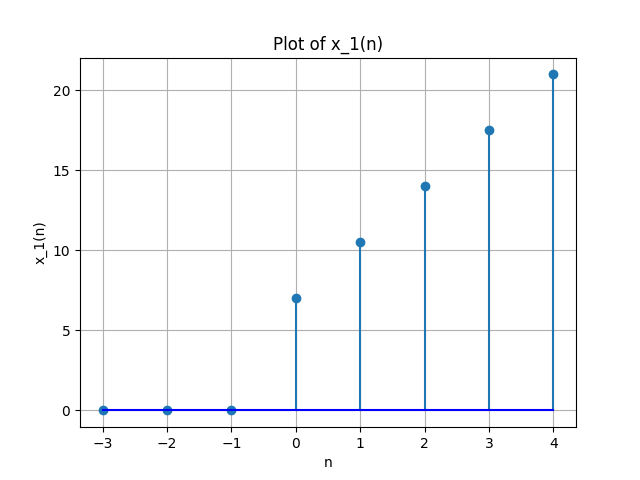
\includegraphics[width=10cm, height=6cm]{graph_1}
\caption{The graph of $x_{1(n)}$ vs n is shown above.}\\
\label{graph:1}

\\Now , putting this $x_{1(n)}$ in $\eqref{eq:3}$ , we obtain \\
\begin{align}
     \sum_{n=-\infty}^{\infty}(x_{1(0)} + \dfrac{7n}{2})u_{(n)}Z^{-n} =X_{1(z)}
\end{align}
\begin{align}
\sum_{n=-\infty}^{\infty}(7 + \dfrac{7n}{2})u_{(n)}Z^{-n} =X_{1(z)}
\end{align}
For the \textbf{region of convergence}\\
$X_{1(z)}$ = convergent $\forall$ z $\epsilon$(-\infty,-1)U(1,\infty)
\\

This can be proved from ratio test . \\
We now calculate the sum using the formula for gp and agp(Assuming $(k-1)^{th}$ term is the last term and also where $x_{1(0)}$ is the first term), we obtain.\\

\begin{align}
   \notag 7(1-z^k)(z^k(1-z))^{-1}+
   \\ \notag(7(z^k-1)z)(2z^k(z-1)^2)^{-1}-\\ (7kz)(2z^{k+1}(z-1))^{-1}=X_{1(z)}
\end{align}
\graphicspath{ {figs/} }
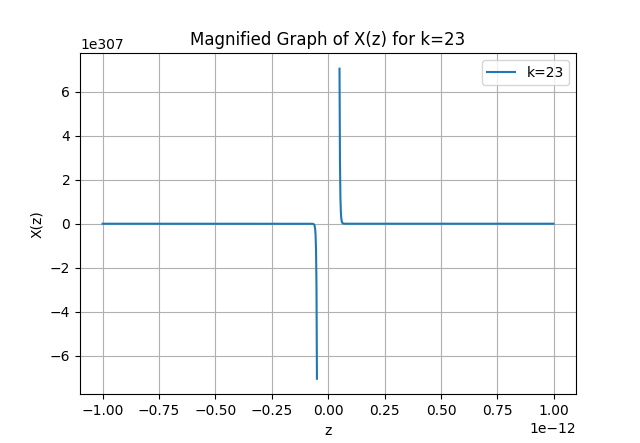
\includegraphics[width=9cm, height=6cm]{Figure_2}
\caption{Above is the graph of $X_{1(z)}$ vs z}\\
\label{graph:2}
\\

It is told to replace $S_n$*u$_{(n)}$ with x(n) \\and therefore calculate X(Z). The equation $\eqref{eq:1}$ and calculate the general form of X(Z) .
It is known that\\
\begin{align}
 \sum_{n=-\infty}^{\infty} Z^{-n}x(n) = X(Z)\label{eq:3}
 \end{align}

Putting the equation $\eqref{eq:1}$ in $\eqref{eq:3}$\\
\begin{align}
    \sum_{n=-\infty}^{\infty} u_{(n)}Z^{-n}\dfrac{n}{2}(2a + (n-1)d) = X(Z) \label{eq:4}
\end{align}
Writing another equation by multiplying $\eqref{eq:4}$ with Z, we get
\begin{align}    
\sum_{n=-\infty}^{\infty} u_{(n)}Z^{-n+1}\dfrac{n}{2}(2a + (n-1)d) = ZX(Z)\label{eq:5}
\end{align}
Now we subtract $\eqref{eq:4}$ from $\eqref{eq:5}$ by displacing it with one term , i.e we subtract the first term of $\eqref{eq:4}$ \\from the second term of $\eqref{eq:5}$ and so on.\\
By simplifying this, we get
\begin{align}
    \sum_{n=-\infty}^{\infty} (a-\dfrac{d}{2})u_{(n)}Z^{-n}+\dfrac{n}{2}dZ^{-n} = ZX(Z)-X(Z)
\end{align}
The first part is a GP and the second part is an AGP. Since the nature of Z is not known, we calculate the general sum for finite terms(Assuming k) and then use it for each bit.\\
Calculating the individual sums, we get
\begin{align}
\notag((a-\dfrac{d}{2})Z^{1-k}((Z^{k}-1))(Z-1)^{-1}+ \\ \notag (d)(2Z^{k-2})^{-1}(Z^{k-1}-1)^(2(Z-1)^{2})^{-1}-\\ \notag(d(k-1))(2(Z-1)Z^{k-1})^{-1})(Z-1)^{-1}\\ =X(Z)
\end{align}
By substituting the respective values of k,a,d we obtain the following:\\
\item 
\begin{align}
    \notag X(Z)=((\dfrac{21}{4})Z^{-22}((Z^{23}-1))(Z-1)^{-1}+\\
    \notag 7(4Z^{21})^{-1}(Z^{22}-1)(2(Z-1)^{2})^{-1}-\\
     \notag(7(22))(4(Z-1)Z^{22})^{-1})(Z-1)^{-1} 
\end{align}








\item[(ii)]
\vspace{0.5cm}
Based on the analysis of the previous bit, we observe that in this bit \\ a=34 , d=-2
For calculating the number of terms, we use the formula (\eqref{eq:2}\\
Substituting the values, we get
\begin{align}
     10 = 34 + (n-1)(-2)
     \end{align}
Solving this yields n=13\\
For calculating $X_{2(z)}$, we first write $x_{2(n)}$ ( here x(0) is 34)\\
\begin{align}
x_{2(n)} = x_{2(0)} + nd\\
x_{2(n)} = x_{2(0)} -2n
\end{align}
\graphicspath{ {figs/} }
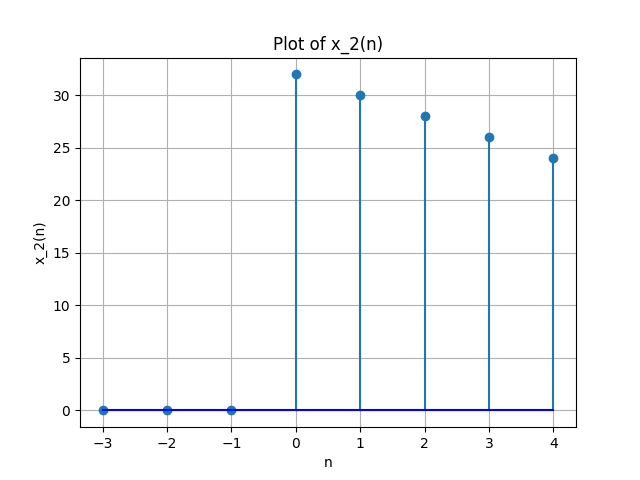
\includegraphics[width=10cm, height=6cm]{graph_2}
\caption{The graph of $x_{2(n)}$ vs n is shown above}\\
\label{graph:3}
\\
Now , putting this value in \eqref{eq:3}, we obtain\\
\begin{align}
\sum_{n=-\infty}^{\infty}(x_{2(0)} -2n)u_{(n)}Z^{-n} =X_{2(z)}
\end{align}
It can be observed that the region of convergence does not change as the nature of the function remains the same as (i)bit\\
For $X_{2(z)}$ , we use the same analogy as in (i)bit to obtain X(z)\\
\begin{align}
   \notag 32(1-z^k)(z^k(1-z))^{-1}-
   \\ \notag(2(z^k-1)z)(z^k(z-1)^2)^{-1}+\\ (2kz)(z^{k+1}(z-1))^{-1}=X_{2(z)}
\end{align}



As For calculating the sum , we use \eqref{eq:1}
\begin{align}
 S_{13} = \dfrac{13}{2}(64+11(-2))
 \end{align}
 Solving this, we get $S_n$= 286.\\\\
 Using the equation(12) , we obtain X(Z) as:\\
  \item 
  \begin{align}      
  \notag X(Z)= (35Z^{-12}((Z^{13}-1))(Z-1)^{-1}-\\
  \notag (Z^{11})^{-1}(Z^{12}-1)(2(Z-1)^{2})^{-1}+\\
  \notag (24)((Z-1)Z^{12})^{-1})(Z-1)^{-1}
    \end{align}


\item[(iii)]  
\vspace{0.5cm}
By using the previous analysis, we can conclude that a=-5, d=-3\\
Again, for n , we use the formula \eqref{eq:2}
\begin{align}
-230= -5+(n-1)(-3)
\end{align}
Solving this yields n=76\\
Now, we write the equation for $x_{3(n)}$ ( given x(0) is -5)
\begin{align}
x_{3(n)} = x_3{(0)} + nd\\
x_{3(n)}=x_3{(0)} - 3n
\end{align}
\graphicspath{ {figs/} }
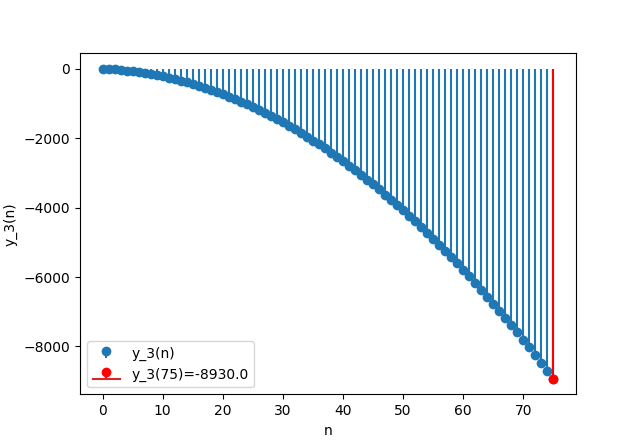
\includegraphics[width=10cm, height=6cm]{graph_3}
\caption{The graph of $x_{3(n)}$ vs n is shown above.}\\
\label{graph:4}
Now , putting this value in \eqref{eq:3}, we obtain\\
\begin{align}
\sum_{n=-\infty}^{\infty}(x_{3(0)} -3n)u_{(n)}Z^{-n} =X_{3(z)}
\end{align}
Again , it can be observed that the region of convergence does not change as the nature of the function remains the same as (i)bit\\
For $X_{3(z)}$ , we use the same analogy as in (i)bit to obtain \\
\begin{align}
   \notag -5(1-z^k)(z^k(1-z))^{-1}-
   \\ \notag(3(z^k-1)z)(z^k(z-1)^2)^{-1}+\\ (3kz)(z^{k+1}(z-1))^{-1}=X_{3(z)}
\end{align}
Now, for the sum we use equation \eqref{eq:1} :\\
\begin{align}
    S_{76}=\dfrac{76}{2}(-10+(76-1)(-3))
    \end{align}
Solving this we obtain $S_{76}$=-8930.\\\\
 Using the equation(12) , we obtain X(Z) as:\\
 \item 
 \begin{align}
 \notag X(Z) =((\dfrac{7}{2})Z^{-75}((Z^{76}-1))(Z-1)^{-1}-\\
 \notag(-3)(2Z^{74})^{-1}(Z^{75}-1)(2(Z-1)^{2})^{-1}+\\
 \notag(-3(75))(2(Z-1)Z^{75})^{-1})(Z-1)^{-1}
 \end{align}
 \\

 \newpage
 
 \begin{center}
\begin{tabular}{ |c|c|c| } 
 \hline
 Parameters & Equations  \\ 
 \hline
  $x_{1(n)}$ &  $x_{1(0)}$ +3.5n\\
  $x_{2(n)}$ & $x_{2(0)}$ -2n\\
  $x_{3(n)}$ & $x_{3(0)}$ -3n\\
 $X_{1(z)}$ &  $7(1-z^k)(z^k(1-z))^{-1}+
    (7(z^k-1)z)(2z^k(z-1)^2)^{-1}-(7kz)(2z^{k+1}(z-1))^{-1}$\\
 $X_{2(z)}$ &  $32(1-z^k)(z^k(1-z))^{-1}-
    (2(z^k-1)z)(z^k(z-1)^2)^{-1}+(2kz)(z^{k+1}(z-1))^{-1}$  \\ 
$Z_{3(z)}$ &  $-5(1-z^k)(z^k(1-z))^{-1}-
    (3(z^k-1)z)(z^k(z-1)^2)^{-1}+(3kz)(z^{k+1}(z-1))^{-1}$ \\
 \hline
\end{tabular}
\end{center}
\caption{ Given above is the list of all parameters used in the analysis so far}.\\


 






\end{enumerate}



 

 






\end{document}
